\chapter{Executive Summary}
\label{ch:dp-execsum}



\section{Introduction}
\label{sec:dp-execsum-introduction}


The \dword{dune} \dword{dp} \dword{detmodule} opens new windows of opportunity for studying neutrinos, a goal it shares with the \dword{spmod}. 
 \dword{dune}'s rich physics program, with discovery potential for \dword{cp} in the neutrino sector and its capability to make significant observations of nucleon decay and astrophysical events is enabled by the exquisite resolution of the \dword{lartpc} detector technique, which the \dword{dp} design further augments. This design improves the \dword{s/n} ratio in the charge readout, reducing the threshold for the smallest observable signals, while also achieving a finer readout granularity.  The \dword{dp} technology enables constructing larger drift volumes, thereby reducing  the quantity of nonactive materials in the \dword{lar}. Constructing and installing the \dword{detmodule} are also simplified by reducing the costs and the number of  building blocks. The readout electronics are fully accessible and replaceable during the entire lifetime of the experiment. Although the physics requirements are identical for both the \dword{sp} and \dword{dp} designs, some aspects of the \dword{dp} design offer augmented performance. 

The basic operating principle is very similar to that of the \dword{sp} design.  Charged particles that traverse the active volume of the \dword{lartpc} ionize the medium while also producing scintillation light.  The ionization electrons drift along an \efield towards a segmented anode where they deposit their charge, and \dwords{pd} pick up the scintillation light. The precision tracking and calorimetry offered by the \dword{dp} technology provides excellent capabilities for identifying interactions of interest while mitigating sources of background.  Whereas the \dword{sp} design has multiple drift volumes, the \dword{dpmod} design allows a single, fully homogeneous \dword{lar} volume with a much longer drift length. This volume is surrounded by a \dword{fc} on the sides and a cathode at the bottom, which together define the drift field. 

The key differentiating concept of the \dword{dp} design is the amplification of the ionization signal in an avalanche process. In the \dword{sp} design, charges drift horizontally to the anode, which consists of a set of induction and collection wire layers immersed in the \dword{lar}. In the \dword{dp} design, electrons drift upward toward an extraction grid just below the liquid-vapor interface. After reaching the grid, an \efield stronger than the drift field extracts the electrons from the liquid up into the gas phase. Once in the gas, electrons encounter micro-pattern gas detectors, called \dwords{lem}, with high-field regions. The \dwords{lem} amplify the electrons in avalanches that occur in these high-field regions. The amplified charge is then collected and recorded on a \twod anode
consisting of two sets of \SI{3.125}{mm}-pitch gold-plated copper strips that provide the $x$ and $y$ coordinates (and thus two views) of an event. Both \dwords{lem} and anode printed circuit boards are produced in units of $50 \times 50\, $cm$^2$. 

The extraction grid, \dword{lem}, and anode are assembled into three-layered sandwiches with precisely defined inter-stage distances and inter-alignment,  which are then connected together horizontally into modular detection units that are \num{9}~m$^2$. These detection units are called \dwords{crp}. The \dwords{crp} integrate the \dwords{lem} and anodes and support the extraction grid. These units can be individually positioned in a horizontal plane a few millimeters beneath the liquid-gas interface, ensuring the extraction grid is completely immersed. 

The argon scintillation light, which at a wavelength of  \SI{127}{nm} is deep in the UV spectrum; it is recorded by an array of \dwords{pmt} located below the cathode.  The \dwords{pmt}, coated with a wavelength-shifting material, shifts the light  closer to the visible spectrum and records the time and pulse characteristics of the incident light.

Two key factors affect the performance of the \dword{lartpc}.  First, the \dword{lar} purity must be high enough to achieve minimum charge attenuation over the longest drift lengths in the \dword{lartpc}.  Thus, the levels of electronegative contaminants (e.g., oxygen, water) must be reduced and
maintained at $\sim$ppt levels.  The \dword{dp} and \dword{sp} designs have slightly different purity requirements (5 ms versus 3 ms minimal electron lifetime) to  cope optimally with the much longer drift of $12~m$ for the \dword{dp}.

Second, the electronic readout of the \dword{lartpc} requires very low noise levels so the signal from the drifting electrons is clearly discernible over the baseline of the electronics.  This requires use of low-noise cryogenic electronics. 

Amplifying the electron signal in the gas phase mitigates the potential effect of these factors on the performance of the \dword{dp} design.  On the other hand this design requires  higher voltages on the cathode, relative to the \dword{sp}, due to the longer drift field. 

\begin{dunefigure}[Principle of the \dual readout]{fig:figure-label-DPprinciple}{Principle of the DP readout.}
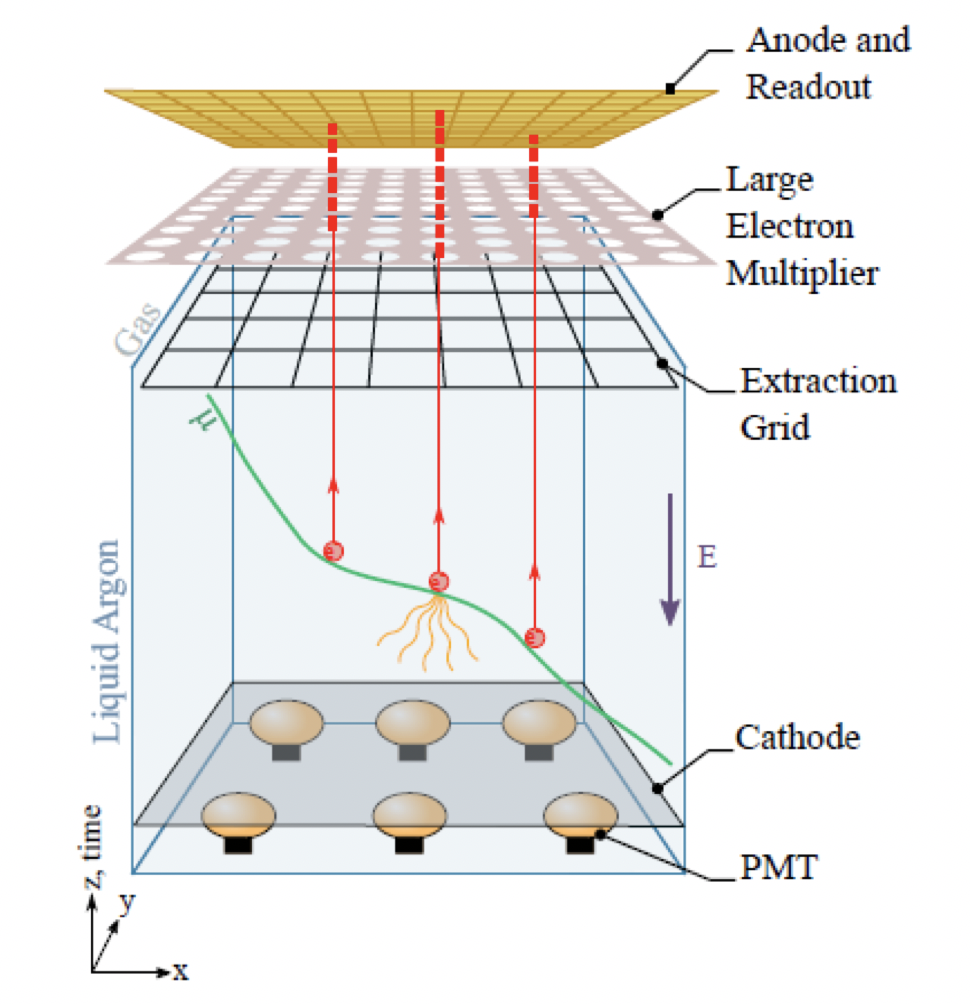
\includegraphics[width=0.6\textwidth]{dualphase-principle}
\end{dunefigure}

%%%%%%%%%%%%%%%%%%%%%%%%%%%%%%%%%%%%%%%%%%%%%%%%%%%%%%%%%%%%%%%%%%%%
\section{Motivation for the \dual Design} 
\label{sec:dp-execsum-design-motivation}

The innovative \dword{dp} design is similar, in many ways, to the \dword{sp} design but implements some unique features and offers several advantages, providing an appealing and complementary approach, as summarized below:

\begin{itemize}
\item Gain on the ionization signal obtained in the gas phase:
\begin{itemize}
\item  leading to a tunable \dword{s/n} and a lower detection threshold, and
\item  compensating for potential charge attenuation due to long drift paths; 
\end{itemize}
\item  Larger fiducial volume, enabling very long drift paths;
\item  Absence of dead material in the \dword{lar} drift volume;
\item  Finer readout pitch (\SI{3}{mm}), implemented in two identical collection views, $x$ and $y$;
\item  Fewer readout channels (\dpnumcrpch for \dword{dp} versus \spnumch for \dword{sp} for a  \nominalmodsize module); 
\item  Fewer construction modules and simpler installation procedures;
\item  Full accessibility and replaceability of the \dword{fe} electronics during the detector operation.
\end{itemize}

The \dword{dp} design features maximize the capability of the experiment and cope with the unprecedented scale of the \dwords{detmodule} and the deep underground location where construction will occur.

Among the features driven by the underground location of the experiment, all detector components are sized to fit within the constraints of the \dword{surf} shafts and access pathways. The \dword{crp} modules are essentially planar objects with a surface of \num{3}\,$\times$\,\SI{3}{m$^2$}. All the other detector 
components (\dword{fc} and cathode modules) are  designed to stay within this envelope. The relatively small number of detector elements makes the underground installation easier.

A drift time of several milliseconds is typical for ionization charge to arrive at the anode wires after drifting several meters.  This lengthy duration, as well as aspects of the \dword{dune} physics program looking for rare and low-energy processes, makes the deep underground location essential for the \dword{dpmod}.  The \SI{1.5}{km} overburden of earth will greatly reduce the rate of cosmic rays reaching the active volume of the \dword{dpmod}, enhancing the ability to search for rare and low-energy signatures without the influence of cosmic-induced backgrounds.  


%%%%%%%%%%%%%%%%%%%%%%%%%%%%%%%%%%%%%%%%%%%%%%%%%%%%%%%%%%%%%%%%%%%%
\section{Overview of Dual-Phase Design}
\label{sec:dp-execsum-description}

This \dword{dp} design implements a \dword{dp} \dword{lartpc} augmented with a light-readout system.  \dword{dp} refers to the extraction of ionization electrons at the interface between the liquid and gas argon and their amplification and collection in the gas phase.

The \dword{dpmod} features a  \dpactivelarmass{} active mass \dword{lartpc}, with all associated cryogenics, electronic readout, computing, and safety systems. The \dword{dpmod} is designed to maximize the active volume within the confines of the membrane cryostat while minimizing dead regions and the presence of dead materials in the drift region. The detector is built as a single active volume \dptpclen long, \dptpcwdth wide and \tpcheight high, with the anode at the top, the cathode near the bottom, and an array of \dwords{pmt} at the bottom underneath the cathode. The active volume (see Figure~\ref{fig:DPdet1}) is surrounded by the \dword{fc}. The ionization electrons in the liquid phase drift  in a uniform \efield towards the anode plane at the top of the active volume. This is made by an array of \num{80} independent \dword{crp} modules, \num{3}\,$\times$\,\SI{3}{m$^2$} each. The cryogenic \dword{fe} electronics is  installed in the \dwords{sftchimney} on the roof of the cryostat. Mo active electronics elements are in the cryostat volume other than the \dword{pmt} bases. The proposed design optimally exploits the cryostat volume of \cryostatwdth{}(w)\,$\times$\,\cryostatht{}(h)\,$\times$\cryostatlen{}(l) with an anode active area of \dptpcwdth{}\,$\times$\,\cryostatlen{} and a maximum drift length of \dpmaxdrift{}, corresponding to an active \dword{lar} mass of \dpactivelarmass  (\dpfidlarmass fiducial). 

The detector elements (\dwords{crp}, \dword{fc}, and cathode) are modular so their production can proceed in parallel with  construction of the \dword{dune} caverns and cryostats; they are sized to conform to the access restrictions for transport underground. Table~\ref{tab:dune-dp-parameters} summarizes  the high-level parameters of the \dword{dpmod} while Figure~\ref{fig:DPdet1} shows the \dword{dpmod}'s main components.

\begin{dunetable}[Dual-phase module parameters]{lll}{tab:dune-dp-parameters}{\Dword{dpmod} parameters.}
Parameter & Value & Note \\ \toprowrule
Cryostat \dword{lar} Mass & \larmass & \\ \colhline 
Active \dword{lar} Mass & \dpactivelarmass & \\  \colhline 
Active height & \tpcheight & \\  \colhline 
Active length & \dptpclen & \\  \colhline 
Maximum drift & \dpmaxdrift & \\ \colhline 
Number of \dwords{crp} &\dptotcrp & \\  \colhline 
Number of \dword{crp} channels & \dpnumcrpch & \\ \colhline 
Number of \dword{pmt} channels & \dpnumpmtch & \\ 
\end{dunetable}

\begin{dunefigure}[Diagram of the \dword{dpmod}]{fig:DPdet1}
  {The \dword{dpmod} with cathode, \dwords{pmt}, \dword{fc}, and anode plane with \dwords{sftchimney}.}
  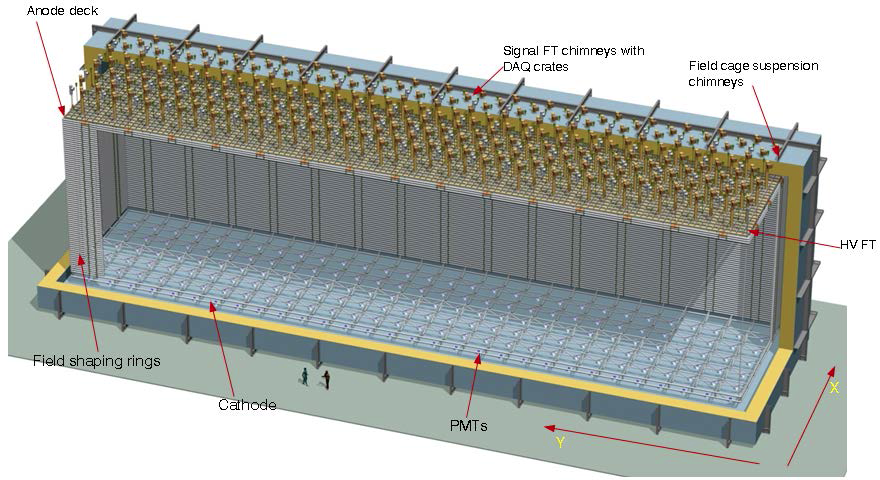
\includegraphics[width=0.9\textwidth]{DUNE-CDR-detectors-volume-optim.png}
\end{dunefigure}

Extracting electrons from the liquid to vapor phase can be done thanks to the submersed horizontal extraction grid integrated in each \dword{crp} structure. A \dword{crp} unit includes \dpswchpercrp (0.5~m$\times$0.5~m) \dword{lem}/anode sandwiches, providing tunable amplification and charge collection on two independent views organized in strips \SI{3}{m} long with \dpstrippitch pitch. Each \dword{crp} had \dpchpercrp readout channels. Signals in each \dword{crp} unit are collected via three \dwords{sftchimney} hosting the \dword{fe} cards with the cryogenic \dword{asic} amplifiers (\dpchperchimney channels/chimney), which are accessible and replaceable without contaminating the pure \dword{lar} volume. Each \dword{sftchimney} is coupled to a microTCA crate to provide signal digitization and  \dword{daq}. These crates are connected  via optical fiber links to the \dword{daq} back-end. The total number of readout channels  per \nominalmodsize module is \dpnumcrpch.

Each \dword{crp} unit is independently suspended by three stainless steel ropes. The vertical level of each \dword{crp} unit can be automatically adjusted for \dword{lar} level via three suspension \fdth{}s. The stainless steel ropes are operated by step motors located outside the suspension \fdth{}s. Slow-control \fdth{}s,  one per \dword{crp} unit, are used for level meters and temperature probes readout,   for pulsing calibration signals, and to apply \dword{hv} bias on the two sides of the \dwords{lem} and on the extraction grid. The \dword{fc} and the anode are constructed of modules similar in dimension to those in \dword{pddp}.

The number of components and corresponding parameters for the \dpactivelarmass \dword{dpmod} are summarized in Table~\ref{tab:DP_numbers}.

\begin{dunetable}[Quantities of items or parameters for the \dword{dpmod}]{ll}{tab:DP_numbers}{Quantities of items or parameters for the \dpactivelarmass  \dword{dpmod}.}  Item & Number or Parameter    \\ \toprowrule
Anode plane size & W = \dptpcwdth, L = \dptpclen \\ \colhline
\dword{crp} unit size & W = \SI{3}{m}, L = \SI{3}{m}  \\ \colhline
\dword{crp} units & \num{4}\,$\times$\,\num{20} = \dptotcrp \\ \colhline
\dword{lem}-anode sandwiches per \dword{crp} unit & \dpswchpercrp \\ \colhline 
\dword{lem}-anode sandwiches (total) & \dpnumswch \\ \colhline
\dword{sftchimney} per \dword{crp} unit & \num{3} \\ \colhline
\dword{sftchimney} (total) & \num{240} \\ \colhline
Charge readout channels / \dword{sftchimney} & \num{640}  \\ \colhline
Charge readout channels (total) & \dpnumcrpch \\ \colhline
Suspension \fdth per \dword{crp} unit & \num{3}  \\ \colhline
Suspension \fdth{}s (total) & \num{240}  \\ \colhline
Slow Control \fdth{}s (total) & \num{80} \\ \colhline
\dword{hv} \fdth & \num{1}  \\ \colhline
\dword{hv} for vertical drift & \dptargetdriftvoltpos \\ \colhline
Voltage degrader resistive chains & \num{12} \\ \colhline
Cathode modules & \num{15}  \\ \colhline
Field cage rings & \num{199}     \\ \colhline
Field cage modules (\SI{4}{m}$\times$\SI{12}{m}) & \num{36}  \\ \colhline
\dwords{pmt} (total) & \dpnumpmtch (\num{1}/m$^2$) \\ 
\end{dunetable}

A number of factors make the \dword{dp} \dword{tpc} concept, as described in this chapter, well suited to large detector sizes like the \dword{dpmod}.
In this design,the charge amplification in the \dwords{crp} compensates for the charge attenuation on the long drift paths.  This configuration also simplifies
construction by optimally exploiting the long vertical dimensions of the cryostat, providing a large homogeneous fiducial volume  free of embedded passive materials (effectively increasing the detector size), reducing the number of readout channels,  and ultimately reducing costs.  

The \dwords{crp} collect the charge projectively,  with practically no dead region, and read the signals out  in two collection views, eliminating the need for  induction views,  which  simplifies reconstruction of complicated topologies. The tunable high \dword{s/n} provides operative margins for the noise and electron lifetime conditions and lowers the threshold on the minimum detectable energy depositions.

The \dword{dpmod} design benefited much from the production and testing experience accumulated during several years for \dword{pddp} which has now been completely installed and is being commissioning (see Figure~\ref{fig:dp-execsum-pddp}). 

\begin{dunefigure}[Diagram of the \dword{dpmod}]{fig:dp-execsum-pddp}
  {Inner view of protoDUNE dual-phase after completely installing the \dwords{crp}, \dwords{fc}, and cathode.}
  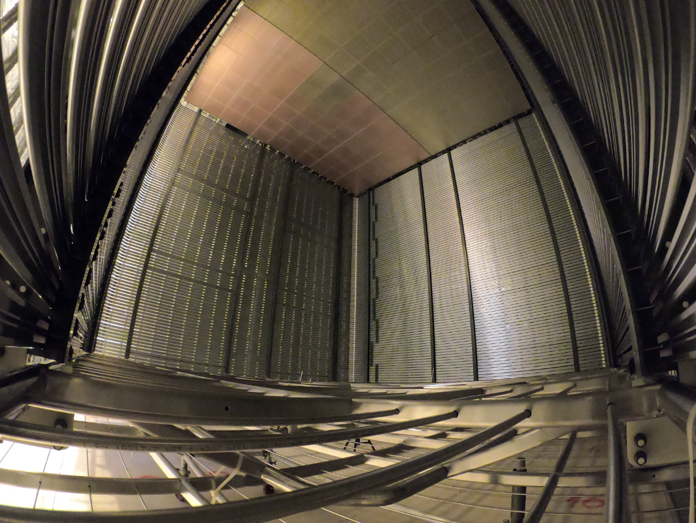
\includegraphics[width=0.7\textwidth]{protodune-dp.png}
\end{dunefigure}

In particular, the charge readout electronics design and the related production and \dword{qa}/\dword{qc} chains correspond exactly to those foreseen for  \dword{dpmod}. The \dword{lem}-anode sandwich production and characterization chains, as well as the ones for the  \dwords{pmt},  are also representative of what should be set up for  \dword{dpmod}. The \dword{crp} underwent detailed test procedures in a dedicated cold-box set up to check their \dword{hv} stability and planarity in the operational conditions across the \dword{lar} surface.

The scope of a \dword{dpmod} includes the design, procurement, fabrication, testing, delivery, installation, and commissioning of the detector components, which is organized in detector consortia, specific to \dword{dp} or jointly with \dword{sp}. 

\begin{itemize}
\item \dword{crp}, including extraction grid, \dword{lem}, and anode and readout planes (\dword{dp} consortium);
\item Analog and digital electronics and \dword{sftchimney} (\dword{dp} consortium); 
\item \dword{pds} (\dword{dp} consortium);
\item Cathode, \dword{fc}, and \dword{hv} system (joint \dword{sp}-\dword{dp} consortium);  
\item Slow-control (joint \dword{sp}-\dword{dp} consortium); 
\item Back-end \dword{daq} system (joint \dword{sp}-\dword{dp} consortium).
\end{itemize}


%%%%%%%%%%%%%%%%%%%%%%%%%%%%%%%%%%%%%%%%%%%%%%%%%%%%%%%%%%%%%%%%%%%%%%
\section{Detector Systems}
\label{sec:dp-execsum-systems}

%%%%%%%%%%%%%%%%%%%%%%%%%%%%%%%%%%%
\subsection{Charge Readout Planes}
\label{sec:dp-execsum-crp}

An extraction efficiency of \num{100}\,\% of the electrons from the liquid to the gas phase is achieved with an \efield of the order of \SI{2}{kV/cm} across the liquid-gas interface, applied between an  extraction grid submersed in the liquid and charge amplification  devices situated in the ultra-pure argon gas. 

These amplification devices, called \dwords{lem}, are horizontally  oriented \SI{1}{mm}-thick printed  circuit boards with electrodes on the top and bottom surfaces. They are drilled through with many holes that collectively form a micro-pattern structure;  when a \SI{3}{kV} potential difference is applied across the electrodes, the ionization electrons are amplified by avalanches (Townsend multiplication) occurring in the  pure argon gas in this micro-pattern structure due to the high \efield (\SI{30}{kV/cm}).

The use of avalanches to amplify the charges in the gas phase increases the \dword{s/n} ratio by at least one order of magnitude with the goal of achieving a nominal gain of 20 or more, significantly improving the event reconstruction quality. The requirement on the minimal \dword{crp} gain is set to 6.  The gain also lowers the threshold for small energy depositions and provides a better resolution per volumetric pixel (voxel) compared to an \dword{sp} \dword{lartpc}.  The charge is collected in a finely segmented \twod ($x$ and $y$) readout anode plane at the top of the gas volume and fed to the \dword{fe} electronics.   

The  collection, amplification, and readout components are combined in an array of independent (layered) modules called \dwords{crp}. A \dword{crp} comprises several \num{0.5}\,$\times$\,\SI{0.5}{m$^2$} units, each of which is composed  of a \dword{lem}-anode sandwich.  These units are embedded in a mechanically reinforced frame of FR-4 and iron-nickel invar alloy. This design guarantees the planarity requirements over the \dword{crp} span in spite of the temperature gradient present in the gas phase and possible sagging effects of the three suspension points. The \dword{crp} structure also integrates  the submersed extraction grid, which is an array of $x$ and $y$ oriented stainless steel wires, \SI{0.1}{mm} in diameter, with \dpstrippitch pitch. Thicknesses and possible biasing voltages for the different layers are indicated in Figure~\ref{fig:CRP_struct}.

\begin{dunefigure}[Thicknesses and HV values for electron extraction from liquid to gaseous Ar]{fig:CRP_struct}
{Thicknesses and \dword{hv} values for electron extraction from liquid to gaseous argon, their  multiplication by \dwords{lem}, and their collection on the $x$ and $y$ readout anode plane. The \dword{hv} values are indicated for a drift field of \SI{0.5}{kV/cm} in \dword{lar}.}
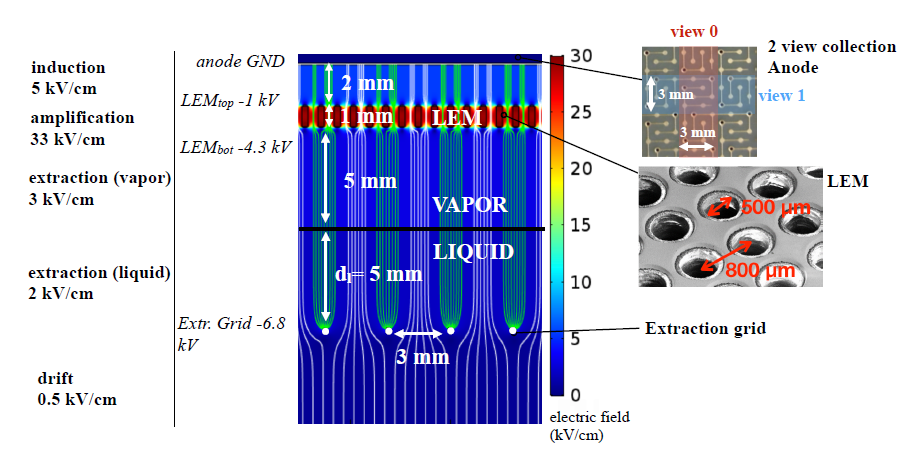
\includegraphics[width=0.8\textwidth]{CRP_gaps.png}
\end{dunefigure}

Each \dword{crp} is independently suspended by three stainless-steel ropes linked to the top deck of the cryostat. This suspension system allows adjustment of the \dword{crp} distance and parallelism with the \dword{lar} surface and keeps the extraction grid immersed. A \dword{crp} provides an adjustable charge gain (with a minimal required gain of \num{20}) and two independent, orthogonal readout views, each with a pitch of \dpstrippitch.  The \dword{lem}/anode sandwiches  in the same \dword{crp} unit are interconnected with short, flat cables, so each readout channel corresponds to a total strip length of \SI{3}{m}. Combined with the time information coming from the \dword{lar} scintillation readout by the \dword{pmt} arrays ($t_0$), a \dword{crp} provides \threed track imaging with $dE/dx$ information.  The \dwords{crp} and their components are described in Chapter~\ref{ch:fddp-CRP}.

The typical amplification achieved by this design, approximately 20, improves the \dword{s/n} ratio and thus compensates for charge losses that occur along the very long drift paths due to the presence of  electronegative impurities. Given the longer drift length, this design requires \dword{lar} to have slightly higher purity than the reference design  (\SI{5}{ms} electron lifetime) to cope with the possibility of operating as well with a minimal drift \efield (\SI{250}{V/cm}) requirement in case the \dwords{crp} also yield a minimal requirement gain of \SI{6}). The required level of purity can be reached by starting from  commercially available ppm-level bulk argon and filling a non-evacuated vessel, as already demonstrated by \dword{pdsp}, which has already achieved up to \SI{7}{ms} electron lifetimes.

For instance, given an electron lifetime of \SI{5}{ms} corresponding to the minimal requirement,  a drift field of \SI{0.5}{kV/cm} and an \dword{lem} gain of \num{20}, \dword{s/n} ratio would be more than  \num{95}:\num{1} for tracks up to \SI{6}{m} from the anode while reaching  \num{45}:\num{1} for  \dword{mip} tracks that are \dpmaxdrift from the anode. This last figure becomes  \num{22}:\num{1} for  \dword{mip} tracks that are \dpmaxdrift from the anode for a drift field reduced to  \SI{0.25}{kV/cm} and \num{6.6}:\num{1} in case all the detector performance parameters correspond to the minimal requirements (\dword{crp} gain of  \SI{6}).

Feedthroughs other than the signal chimneys connected to the \dwords{crp} and the \dword{crp} slow control and \fdth{}s are planned for the cathode \dword{hv} connection, the \dword{crp} suspension and level adjustment, the \dword{hv}, and signal readout of the \dwords{pmt}, and the monitoring instrumentation (level meters, temperature probes, strain gauges, etc.).

Four \dwords{crp} (two of which are instrumented with \dword{lem}) were built in 2018 and underwent detailed operational tests using a dedicated cold-box set up to check their \dword{hv} stability and planarity in the operational conditions present across the \dword{lar} surface (see Figure~\ref{fig:dp-execsum-crp}). 

\begin{dunefigure}[Diagram of the \dword{dpmod}]{fig:dp-execsum-crp}
  {A  \dword{crp} built for \dword{pddp} undergoing the cold-box test procedure.}
  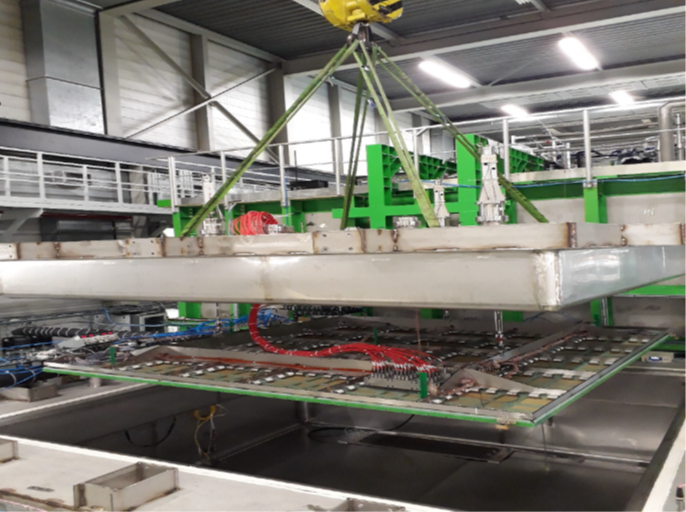
\includegraphics[width=0.7\textwidth]{cold_box_crp.png}
\end{dunefigure}



%%%%%%%%%%%%%%%%%%%%%%%%%%%%%%%%%%%
\subsection{Readout Electronics and Chimneys}
\label{sec:dp-execsum-electronics}

The electrical signals from the collected charges are passed to the outside of the tank via a set of dedicated \dwords{sftchimney}. The chimneys are pipes passing through the top layer of the cryostat insulation and closed at the top and at the bottom by ultra-high-vacuum flanges (warm and cold). The volume inside each \dword{sftchimney} fits tightly in the cryostat inner volume and is filled with nitrogen gas. The bottom (cold) flange of each \dword{sftchimney} is a short distance  from the \dwords{crp} in the cryostat gas volume.

The cryogenic \dword{fe} electronics cards, housed at the bottom of the chimney are plugged into the top side of  the cold flange. The \dword{fe} cards are based on the analog cryogenic preamplifiers implemented in \dword{cmos} \dword{asic} circuits for high integration and large-scale affordable production. 
The \dword{asic} circuits were specially designed, following an R\&D process started in 2006 (the present version was frozen in 2016) to match the signal dynamics of a \dword{dpmod}. Inside the chimneys, the cards are actively cooled to a temperature of approximately \SI{110}{K} and isolated from the \dword{lar} vessel by the cold flange \fdth{}.  The bottom side of the cold flange connects to the \dword{crp} via short flat cables (\SI{0.5}{m} long) in order to minimize the input capacitance to the preamplifiers. Each \dword{sftchimney} collects \num{640} readout channels. 

The \dword{fe} cards are mounted on \SI{2}{m} long blades that slide on lateral guides integrated into the mechanical structure of the chimney, allowing access to and replacement of the analog \dword{fe} electronics from the outside without contaminating the \dword{lar} volume. 
Swapping out the \dword{fe} electronics requires opening a flange at the top of the \dword{sftchimney} and feeding nitrogen into the \dword{sftchimney} in slight over-pressure with respect to the atmospheric pressure.  This operation is quite rapid and straightforward and can be performed while the \dword{detmodule} is taking data. The chimneys act also as Faraday cages, entirely decoupling the analog \dword{fe} electronics 
from picking up possible noise from the digital electronics.   

The digital electronics for the charge digitization system, also the result of a long R\&D process started in 2006 and frozen in 2016, is located 
on the roof the cryostat at room temperature. This makes it possible to use the system as a design standard with infrastructure support for the low-cost, high-speed networking technologies, such as \dword{utca}, used in the telecommunication industries. 

Digitization cards in the \dword{amc} format read \num{64} channels per card. Each \dword{amc} card can digitize all  \num{64} channels at \SI{2.5}{MHz} and compress and transmit this continuous data stream, without zero skipping, over a network link operating at \SI{10}{Gbit/s}. Lossless data compression is particularly effective thanks to the high \dword{s/n} ratio  of \dword{dp}, which limits noise contributions at the level of one \dword{adc} count. Each \dword{sftchimney} is coupled to a \dword{utca} crate that houses in \num{10} \dword{amc} digitization cards in order to read  \num{640} channels and transmit the data via the \dword{mch} switch using a \SI{10}{Gbit/s} optical link connected to the \dword{daq} back-end. This requires \num{240} \dword{utca} crates to read the entire \dword{detmodule}. The \dword{sftchimney} warm flange connects the analog differential signals, via shielded VHDCI cables, to the \dword{amc} digitization cards and also distributes the \dword{lv} and slow control signals to the analog \dword{fe} electronics.  

The light-readout digitization system is also based on \dword{utca} \dword{amc} cards derived from the design of the charge readout and hosting a specific circuitry based on the \dword{catiroc} \dword{asic} to trigger the light-readout. By assuming a \dword{pmt} channel density similar to \dword{pddp}, five \dword{utca} crates are sufficient to read \dpnumpmtch \dwords{pmt}.

The timing synchronization is based on the \dword{wr} standard. Specifically developed timing \dword{mch} connected to a \dword{wr} network ensures the distribution of clock, absolute timing, and trigger information on the backplane of the \dword{utca} crates. The \dword{wrmch} are connected via \SI{1}{Gbit/s} optical fibers to a system of \dword{wr} switches that interconnect the \dword{wr} network. This ensures that the digitization performed by the various \dword{amc} cards is completely aligned; it also refers to the absolute UTC time. 

The \dword{wrgm} switch is connected to a GPS disciplined oscillator unit providing absolute time and the clock frequency reference to the system. The timing system includes \num{16} \dword{wr} switches and \num{240} (charge readout) + \num{5} (light readout) \dword{mch} units.    

The entire readout electronics system has been optimized to support the \dword{dp} features: charge signal dynamics, readout organization via the chimney, the number of readout channels, the high \dword{s/n} ratio, and the possibility of performing continuous data streaming with zero losses to the \dword{daq} back-end. 

Using cost-effective technologies and performing the corresponding R\&D needed to fully exploit these technologies are strategies that have been guiding the R\&D since its beginning to reduce and optimize detector costs.   
This optimization adds to the fact that the number of readout channels is naturally lower for a \dword{dpmod} thanks to the long projective geometry: \dpnumcrpch channels for a \dword{dp} module with \SI{3}{mm} readout pitch to be compared to \spnumch channels for a \dword{sp} module with \SI{5}{mm} readout pitch. 

A fraction (1/20) of the final electronic charge readout system needed for a  \dword{dp} \dword{detmodule}, corresponding to 1/20, was built for \dword{pddp} and deployed on the detector (see Figure~\ref{fig:dp-execsum-FE-ele}).  A subset, six times smaller, already operates successfully  on the $3\times 1 \times 1$ prototype.

\begin{dunefigure}[Diagram of the \dword{dpmod}]{fig:dp-execsum-FE-ele}
  {Front-end charge readout electronics installed on protoDUNE dual-phase.}
  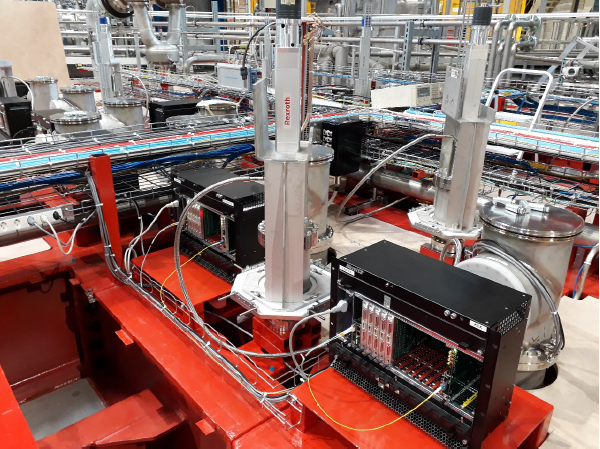
\includegraphics[width=0.7\textwidth]{utca-pddp2}
\end{dunefigure}


%%%%%%%%%%%%%%%%%%%%%%%%%%%%%%%%%%%
\subsection{Cathode, Field Cage, and HV System}
\label{sec:dp-execsum-cathode}

The \dword{hv} system is designed by a common \dword{sp}-\dword{dp} consortium.
The drift field (nominal: E ${\simeq}$ \SI{0.5}{kV/cm}, minimal requirement: E ${\simeq}$ \SI{0.25}{kV/cm}) inside the fully active \dword{lar} volume is produced by applying \dword{hv} to the cathode plane at the bottom of the cryostat and is kept uniform by the \dword{fc}, a stack of \num{199} equally spaced, field-shaping electrodes,  polarized at linearly decreasing voltages from the cathode  voltage to almost ground potential, reached at the level of the \dword{crp}. The electrodes are rectangles made of extruded aluminum profiles (vertical pitch \SI{60.6}{mm}) with rounded corners running horizontally (and stacked vertically) around the active volume. The aluminum profiles are supported and insulated by FRP supporting beams with a pattern of slots where the aluminum profiles can be mounted. Similarly as in \dword{pddp} the profiles are arranged in modules of \SI{4}{m} width including two \dword{frp} supporting columns. These modules are chained together and  hang from the cryostat roof. A chain of \num{6} modules covers the \dpmaxdrift drift. The aluminum profiles of the different modules are joined with short clipping profiles to ensure the electrical continuity over the \dptpclen long horizontal rings. 

The drift cage design shares common structure elements (aluminum profiles and \dword{frp} supporting beams) as the \dword{sp} \dword{fc} design but with a different arrangement (vertically hung structure) to cope with the \dword{dpmod} geometry.

The cathode plane  is suspended from the \dword{fc} and hangs near the  bottom of the cryostat. It consists of 15 adjacent $4~m \times 12~m$ modules to cover the $60~m$ length of \dword{dpmod}. The cathode module design is based on the design used in \dword{pddp} which limits high \efield
regions in its proximity, with modifications to ensure planarity over the longer $12~m$ span of \dword{dpmod} and to implement features to electrically segment the cathode plane.

As shown in  Figure~\ref{fig:dp-execsum-dune-dp-cathode}, each cathode module is constructed of two 12m long trusses made from thin-walled stainless steel tubes with approximately $50~mm$ outer diameter. They can either be prefabricated and transported underground like the large cryostat beams or assembled in the underground cleanroom from sectional parts. The trusses are 2m apart and are connected at both ends to stainless steel tubes that run under the \dword{fc} and form the outer edges of the cathode plane. A total of 122 resistive rods 10mm in diameter are installed at a 10 cm pitch through the holes in the straight upper tubes of the trusses, forming the effective cathode plane. The rods are made from extruded \dword{frp} and wrapped with a layer of the resistive film.

\begin{dunefigure}[A view of a ProtoDUNE-DP cathode module]{fig:dp-execsum-dune-dp-cathode}
{A view of a \dword{pddp} cathode module:  Construction uses a pair of stainless steel trusses as the framework with an array of coated \dword{frp} rods. 
The lower-left inset shows the details of the resistive interconnect and the lifting tab on the cathode truss structure. The upper-right inset is a detailed view of the components in a resistive union.}
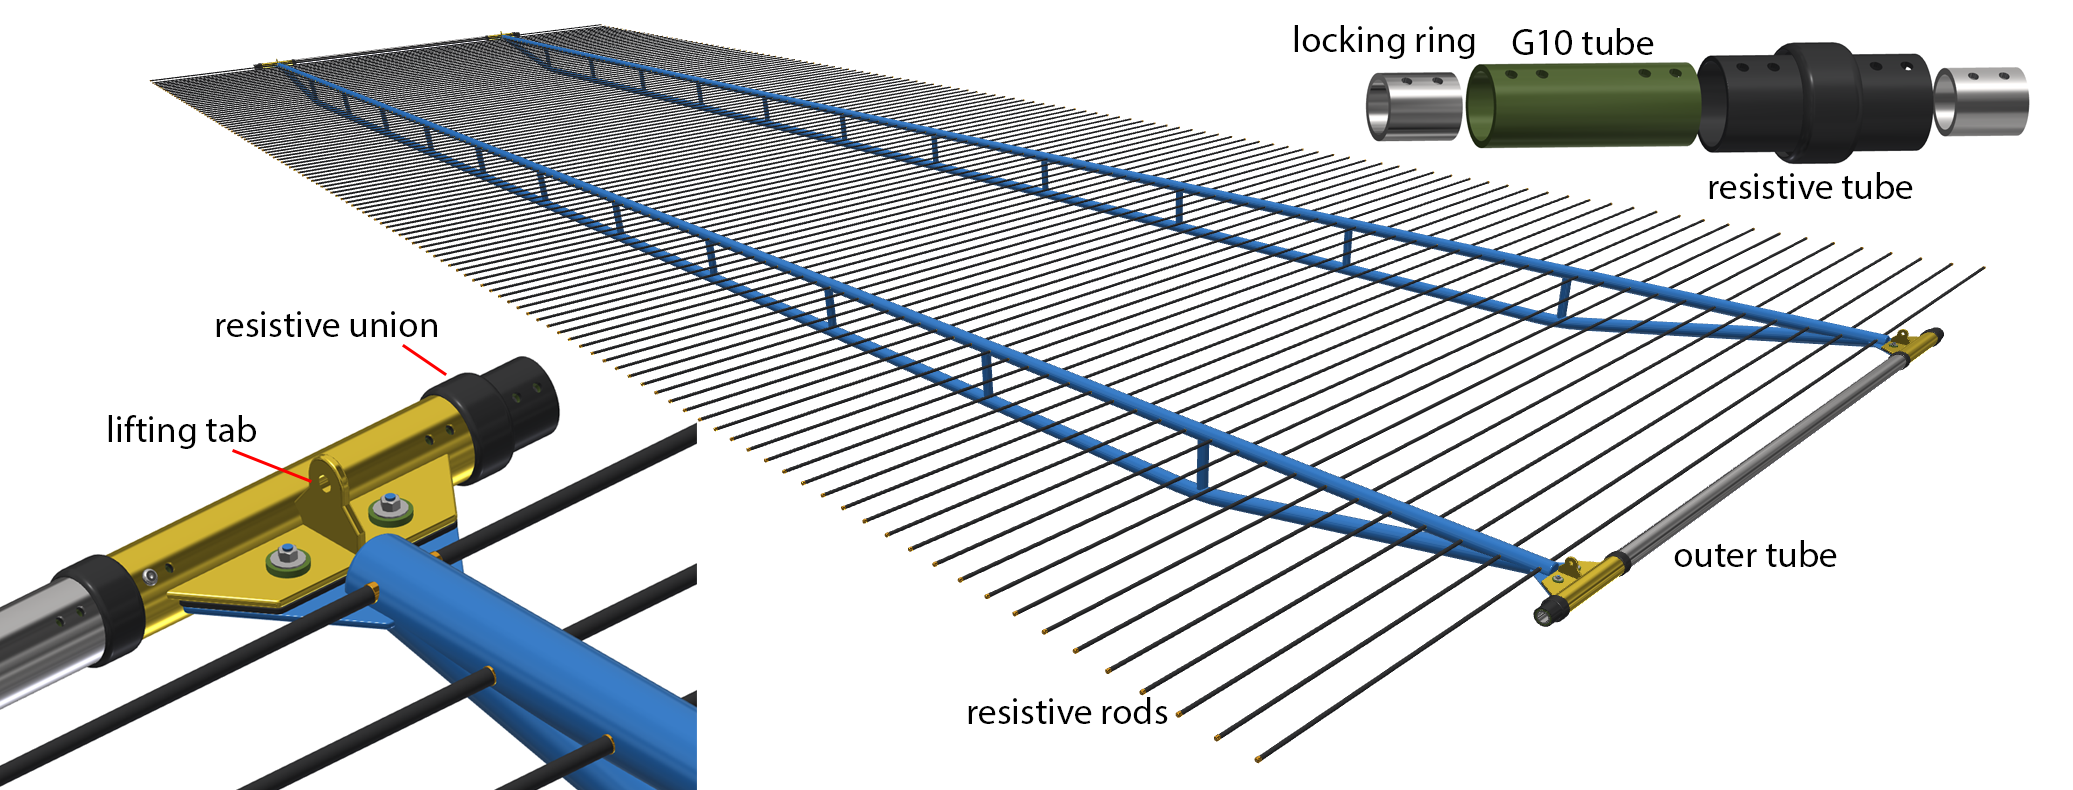
\includegraphics[width=0.9\textwidth]{DP_HVS_cathode_module.png}
\end{dunefigure}

A set of 80 $3~m \times 3~m$ ground grid modules, standing on the cryostat floor, are installed to protect the array of \dword{pmt} from any electric discharge from the cathode.


%%%%%%%%%%%%%%%%%%%%%%%%%%%%%%%%%%%
\subsection{Photon Detection System}
\label{sec:dp-execsum-pd}

The \dword{pds} is based on an array of \dwords{pmt} uniformly distributed below the cathode. Assuming a similar channel density as in \dword{pddp}, this translates to \dpnumpmtch channels. The \dwords{pmt} have a \dword{tpb} coating on the photocathode's external glass surface that shifts the scintillation light from deep UV to visible light. The \dwords{pmt}  sit on the corrugated membrane cryostat floor, on 
mechanical supports that do not interfere with the membrane thermal contraction. 
A single cable provides both \dword{hv} and signal transmission by way of a positively biased base circuitry, thus reducing the required number of \fdth{} channels. Optical fibers provide the calibration system.   Figure \ref{fig:dp-execsum-dppd_3_2} shows the \dword{pmt} with its support base attached to the bottom of the \dword{pddp} cryostat.

\begin{dunefigure}[Hamamatsu R5912-MOD20 \dword{pmt} in \dword{pddp}.]{fig:dp-execsum-dppd_3_2}
{Picture of the cryogenic Hamamatsu R5912-MOD20 \dword{pmt} fixed on the membrane floor of \dword{pddp}. The optical fiber of the calibration system is also visible.}
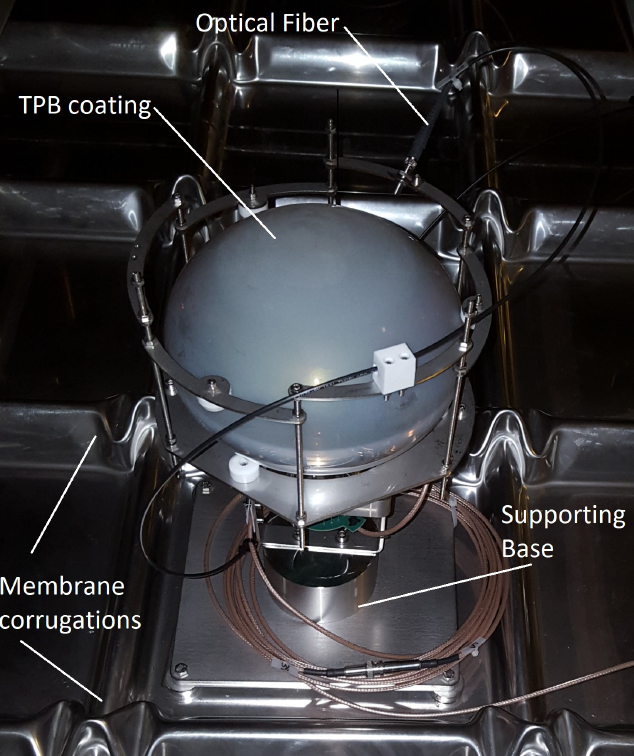
\includegraphics[width=0.42\textwidth]{dp-execsum-pmt1}
\end{dunefigure}

In order to improve the light yield uniformity for signals generated in the top part of the drift volume a system of reflective panels with WLS coating is integrated on the  \dword{fc} walls.


%%%%%%%%%%%%%%%%%%%%%%%%%%%%%%%%%%%
\subsection{Data Acquisition}
\label{sec:dp-execsum-daq}

The Ethernet-based \dword{daq} back-end system is designed by a joint \dword{sp}-\dword{dp} consortium. It connects to 
\SI{10}{Gbits/s} optical links that provide continuous, lossless, compressed data streaming from the \dword{utca} crates, and it has the task of determining the trigger conditions for interesting events like beam, cosmics, and \dword{snb} neutrino interactions. This system also manages recording data to disk. The system can exploit the high \dword{s/n} ratio peculiar to the \dword{dp} design, the availability of the entire data stream without losses, and the possibility of going to lower detection thresholds for \dword{snb} events.

The \dword{dpmod} \dword{daq} is identical to that of the \dword{spmod}. %\fixme{Is the previous sentence correct? It appears to say that the DP module is identical to the DP module. (Anne changed it to SP - good catch.)} 
Although the architecture of the detector readout electronics is different for each technology, the output format of the generated data is common, and both are synchronized to the same global clock signals. The readout data are continuously streamed via \SI{10}{Gbit/s}  optical links by each detector module \dword{fe} electronics system to the \dword{daq}. There they are aggregated, and trigger primitives are constructed based on a common set of algorithms. A final trigger decision is then taken, and depending on the outcome, relevant data time slices are moved to persistent storage. Figure~\ref{fig:dp-execsum-daq-interface-scheme} provides a schematic illustration of these concepts.
  

\begin{dunefigure}[Interface of DP TPC electronics to DAQ]{fig:dp-execsum-daq-interface-scheme}
{Schematic illustration of the interface of \dword{dp} \dword{tpc} electronics to \dword{daq}.}
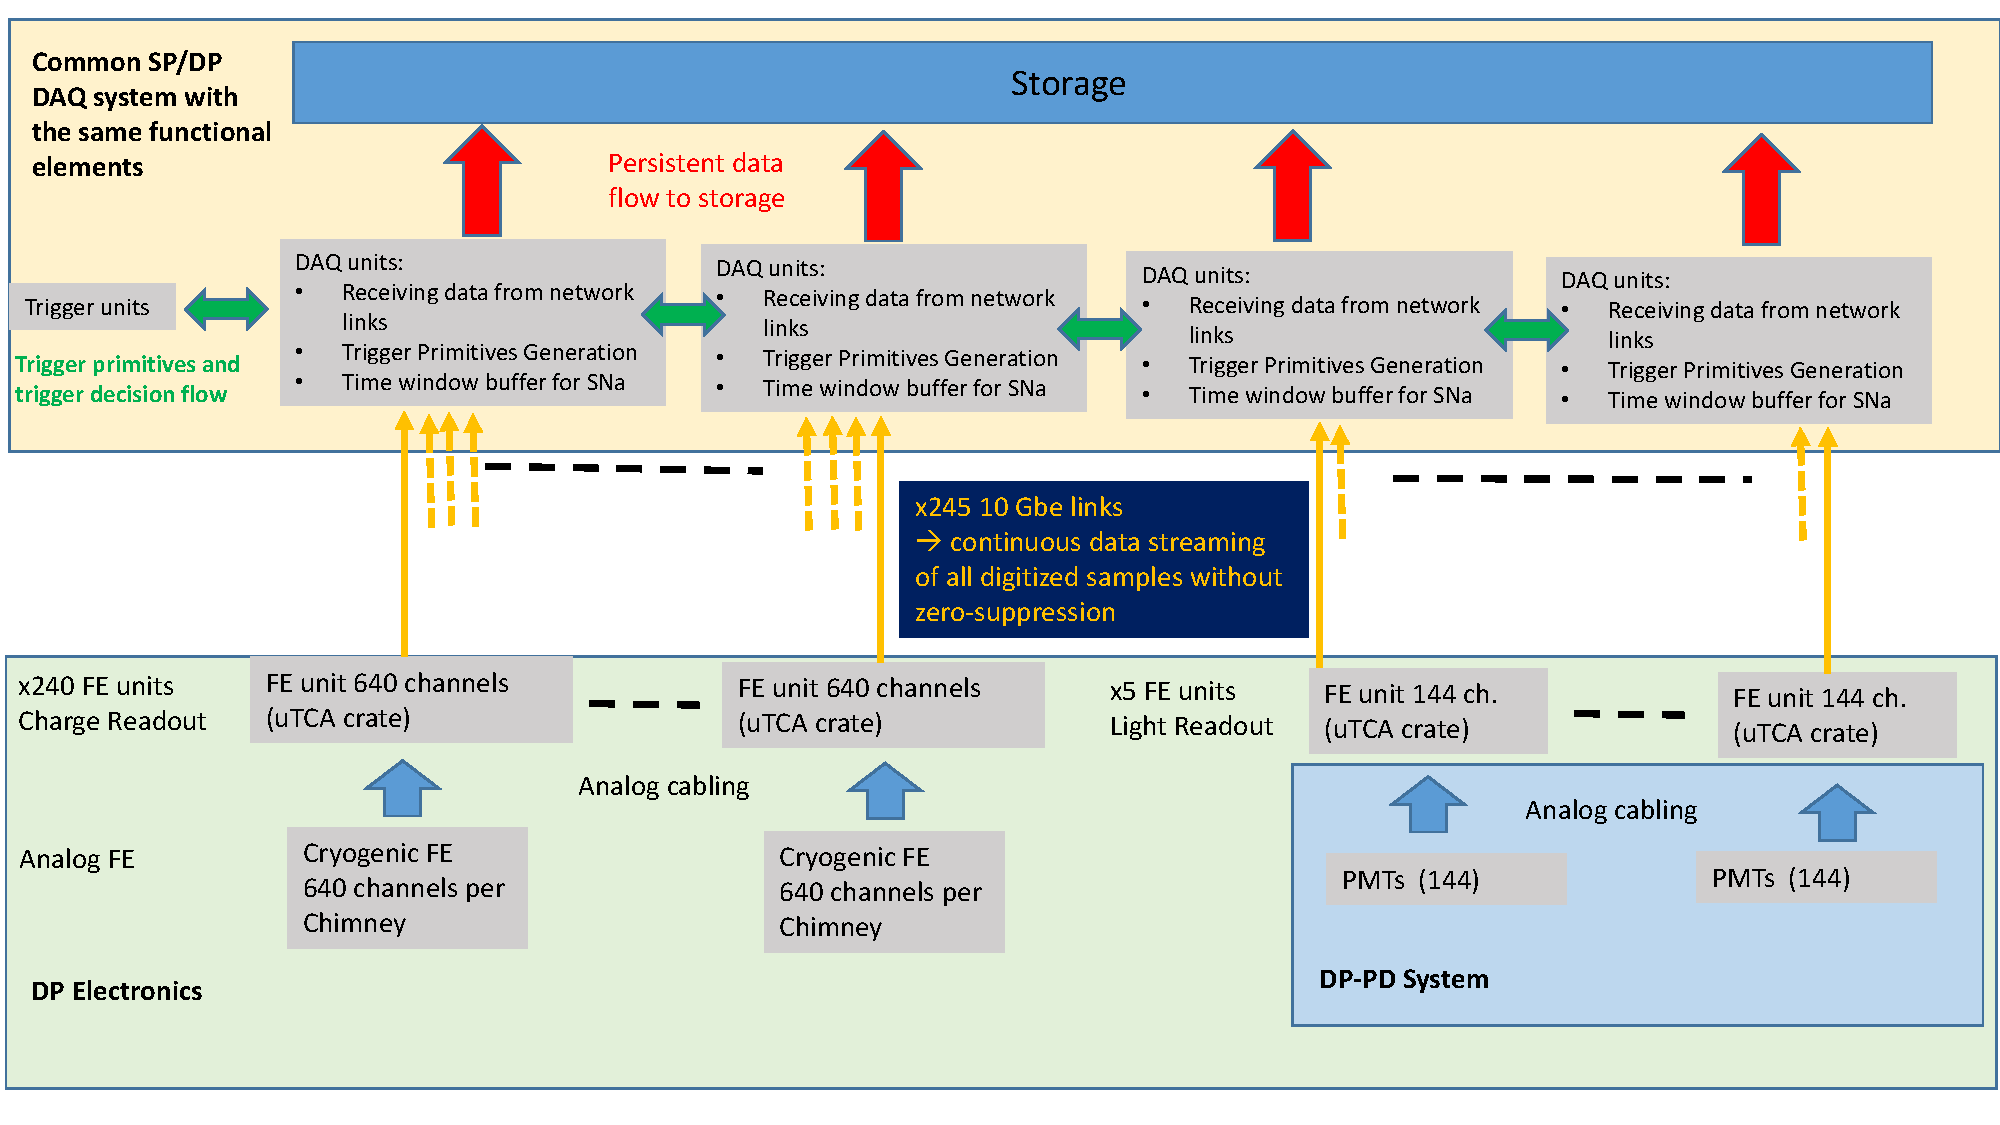
\includegraphics[width=0.95\textwidth]{dp-tpcelec-daq-interface-scheme}
\end{dunefigure}

 We assume that the \dword{daq} back-end system, as for the \dword{sp} design, will comprise a set of event-building and trigger machines, high-performance network elements, and a high-bandwidth distributed storage system based on an array of storage servers operating in parallel. In particular, the \dword{daq} system is expected to

\begin{itemize}
\item Collect the high-bandwidth data volume coming from the data links of the \dword{fe} digitization crates; 
\item Put together the data streams from different crates in \dword{roi} or over the entire detector volume (An \dword{roi} is typically the size of a \dword{pddp} four-\dword{crp} surface because events are contained in such a region.);
\item Process this data flow using an online trigger farm  as a prelude to selecting relevant events to be recorded on disk (both neutrino beam and off-beam events);
\item Produce charge-readout triggers independently of the light-readout triggers and beam-spill information. 
(For \dword{snb} events in particular, the trigger farm would issue triggers over a sliding timing window of approximately \SI{10}{s}  based on the presence of low-energy depositions; the entire content would be dumped to disk.).
\end{itemize}

The \dword{dp} readout architecture can be organized into \num{20} \dwords{roi}, each similar to the \dword{pddp} back-end architecture. Triggers are searched on the level-1 event builder machines, interconnecting multiple \dword{utca} crates, on a sliding windows of \SI{10}{s}  contained in the event builder RAM.

The event builders combine continuous lossless, compressed data (streaming from the charge readout) with beam data and light data to define the window $t_0$ and select disk streams from beam events, cosmics, and \dword{snb} events. Data decompression is necessary on the event builders in order to perform the charge data analysis for trigger definition. Compressed data are kept in memory, while the trigger definition analysis is performed, for further writing to disk from level-2 machines from the output streams: beam, cosmics and proton decay, and \dword{snb}. 

The level-1 event builders exchange trigger primitive data on the network with a global supervisor machine, which then decides what data to write to disk.  The supervisor can order the event builder's memory  windows dumped to disk if a certain number of candidate energy depositions is found from the charge data.  This scheme makes it possible for selected portions of different \dwords{detmodule} to communicate with one another.  
Typically for beam data and cosmic events, the amount of data written to disk can be limited to one or two \dwords{roi}; in some situations, events occur at the border between two \dwords{roi} rather than in a single one.


%%%%%%%%%%%%%%%%%%%%%%%%%%%%%%%%%%%
\subsection{Cryogenics Instrumentation and Slow Controls}
\label{sec:dp-execsum-sc}
The \dword{cisc} system is designed by a joint \dword{sp}-\dword{dp} consortium. 
This system controls the following items:

\begin{itemize}
\item Cryogenic instrumentation: measurements of temperatures (gas and liquid), pressure (gas), liquid level, purity monitors;
\item \dword{crp} instrumentation: temperatures, pulsing system, precision level meters, readout of \dword{crp} stepping motors;
\item Generation and control of \dword{hv} biasing of \dword{lem} and grid;
\item Generation and control of \dword{hv} biasing for the \dwords{pmt} and calibration (via optical pulsing);
\item Slow control of the \dword{utca} crates, analog \dword{fe}\dword{lv} control, charge injection control to preamplifiers;
\item Control of the cathode \dword{hv} biasing system;
\item Alignment survey of \dword{crp} position (via external reference points);
\item Control of the laser system;
\item Analysis of \dword{lar} purity and \dword{lem}  gain calibration.
\end{itemize}

  